\documentclass[12pt,a4paper]{article}
\usepackage[a4paper,margin=19mm]{geometry}
\usepackage{graphicx}
\usepackage{subcaption}
\usepackage{float}
\usepackage{amsmath}
\usepackage{hyperref}
\usepackage{tocloft}
\hypersetup{colorlinks=true,linkcolor=black,urlcolor=blue}
\setlength{\parindent}{0pt}
\setlength{\parskip}{5pt}
\renewcommand{\baselinestretch}{1.05}
\setlength{\cftbeforesecskip}{4pt}
\setlength{\cftbeforesubsecskip}{3pt}
% Increase section title size
\usepackage{sectsty}
\sectionfont{\large}
% Make figure captions slightly larger
\usepackage{caption}
\captionsetup{font=large}

\title{\textbf{EN3160 – Assignment 02}\\Feature Detection and Image Alignment}
\author{\textbf{220701X – Savindu Wickramasinghe}\\Department of Electronic and Telecommunication Engineering\\University of Moratuwa}
\date{}

\begin{document}
\maketitle
\vspace{-8mm}
\tableofcontents
\vspace{4mm}
\begin{center}
{\small Repository: \href{https://github.com/Savidilsh/Fitting-and-Alignment}{\url{https://github.com/Savidilsh/Fitting-and-Alignment}}}
\end{center}

\section{Blob Detection using LoG}
We used the Laplacian of Gaussian (LoG) to locate round sunflower heads in the image. The photo was converted to grayscale, blurred with Gaussians at several scales, and the Laplacian operator was computed. Peaks in this scale-space were taken as blob centers.

	extbf{Parameters:} $\sigma_{min}=3$, $\sigma_{max}=12$, $N_\sigma=30$, threshold = 0.3. Only the lower 60\% of the frame was processed to ignore the sky.

The method found the main sunflower heads while ignoring small, noisy spots. The results show LoG works well for detecting roughly circular features over a range of sizes.

\begin{figure}[H]\centering
\begin{subfigure}{0.45\textwidth}
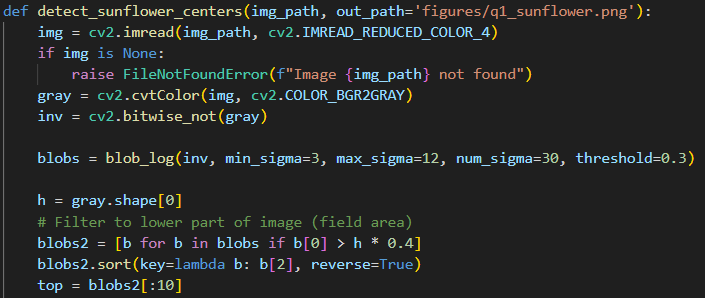
\includegraphics[width=\linewidth]{images/q1_code.png}
\caption{LoG implementation code}
\end{subfigure}\hfill
\begin{subfigure}{0.45\textwidth}
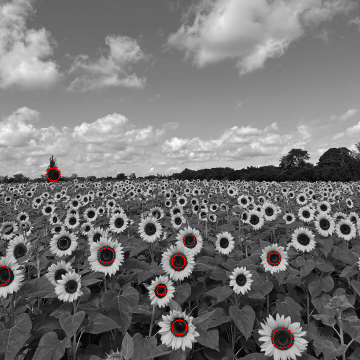
\includegraphics[width=\linewidth]{figures/q1_sunflower.png}
\caption{Detected sunflower blobs}
\end{subfigure}
\caption{Laplacian of Gaussian blob detection results}
\end{figure}

---

\section{RANSAC Line and Circle Fitting}
We created synthetic data that contains points from a line and a circle, both corrupted by Gaussian noise. RANSAC was used to find a robust line fit first, then the remaining points were used to fit a circle.

The final estimates were:
\[
	ext{Line: } a=-0.730,\; b=-0.684,\; d=0.992
\quad
	ext{Circle: } x_0=2.083,\; y_0=2.514,\; r=10.147
\]

RANSAC removed outliers reliably and produced stable model parameters despite the noise.

\begin{figure}[H]\centering
\begin{subfigure}{0.23\textwidth}
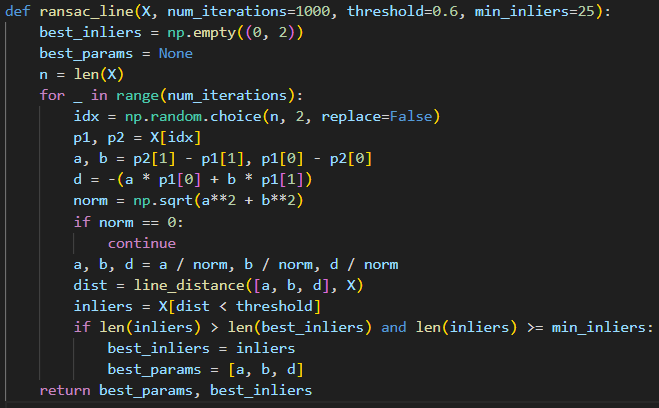
\includegraphics[width=\linewidth]{images/q2_1_code.png}
\caption{Line fitting code}
\end{subfigure}
\begin{subfigure}{0.23\textwidth}
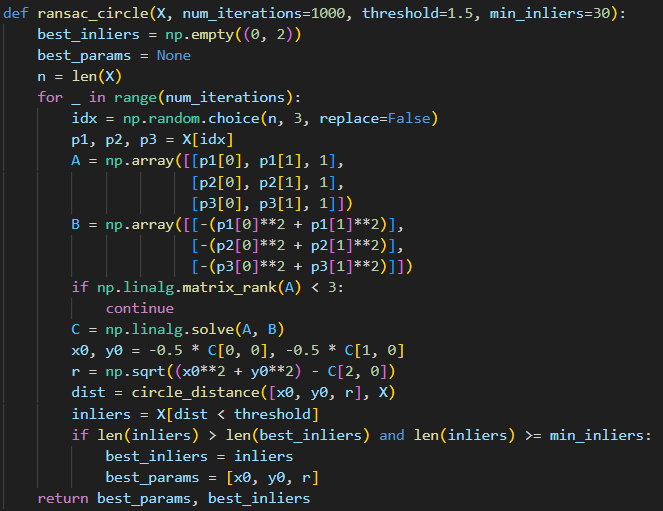
\includegraphics[width=\linewidth]{images/q2_2_code.png}
\caption{Circle fitting code}
\end{subfigure}
\begin{subfigure}{0.23\textwidth}
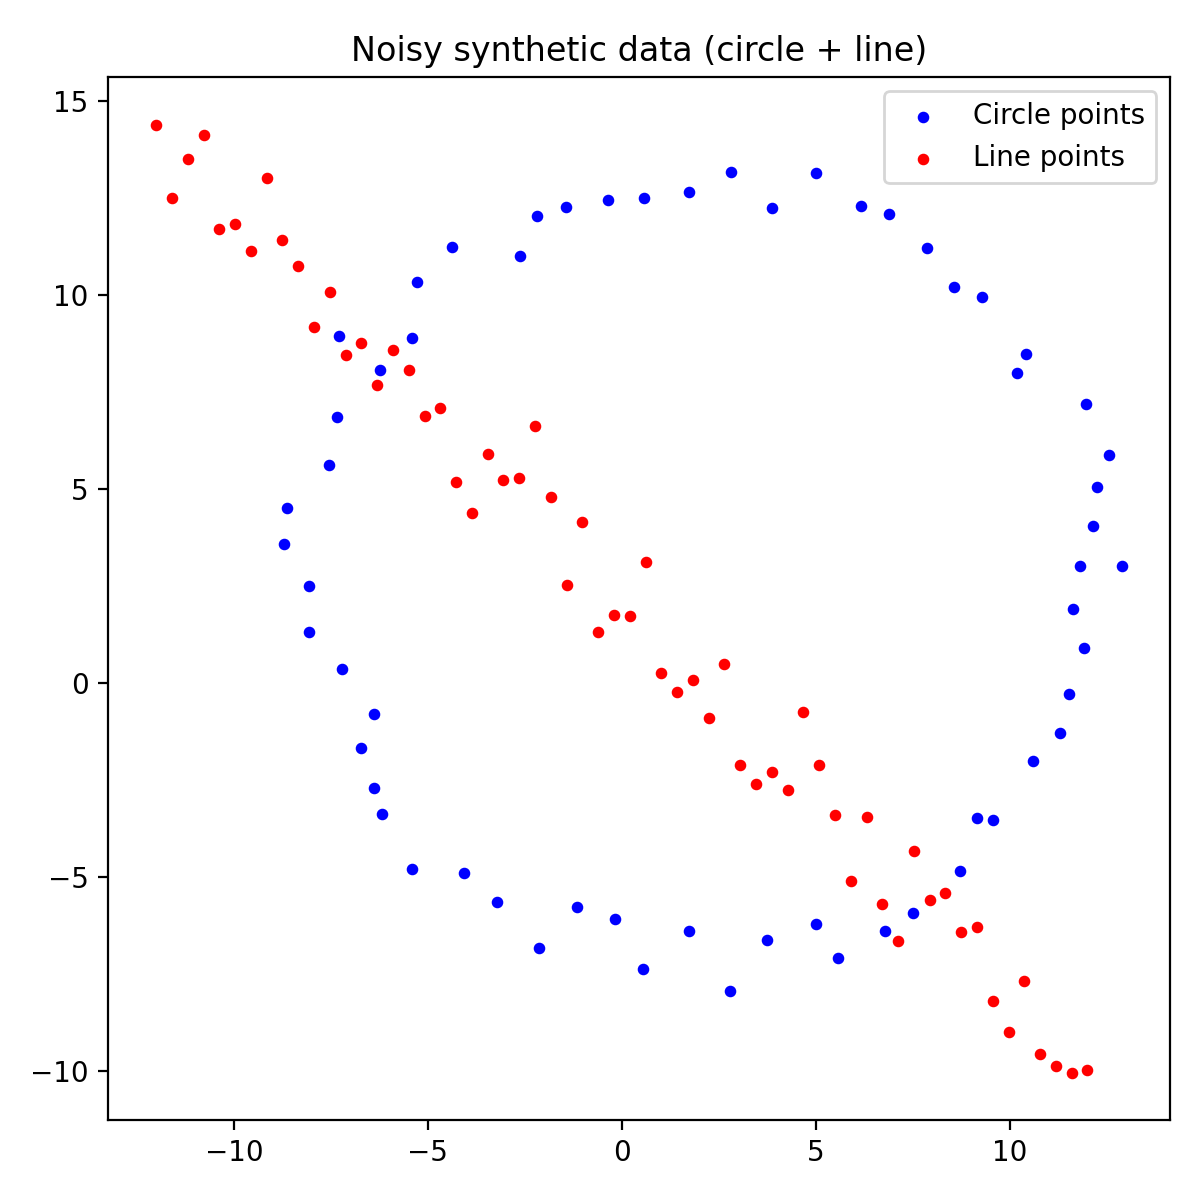
\includegraphics[width=\linewidth]{figures/q2_noisy_data.png}
\caption{Noisy synthetic data}
\end{subfigure}
\begin{subfigure}{0.23\textwidth}
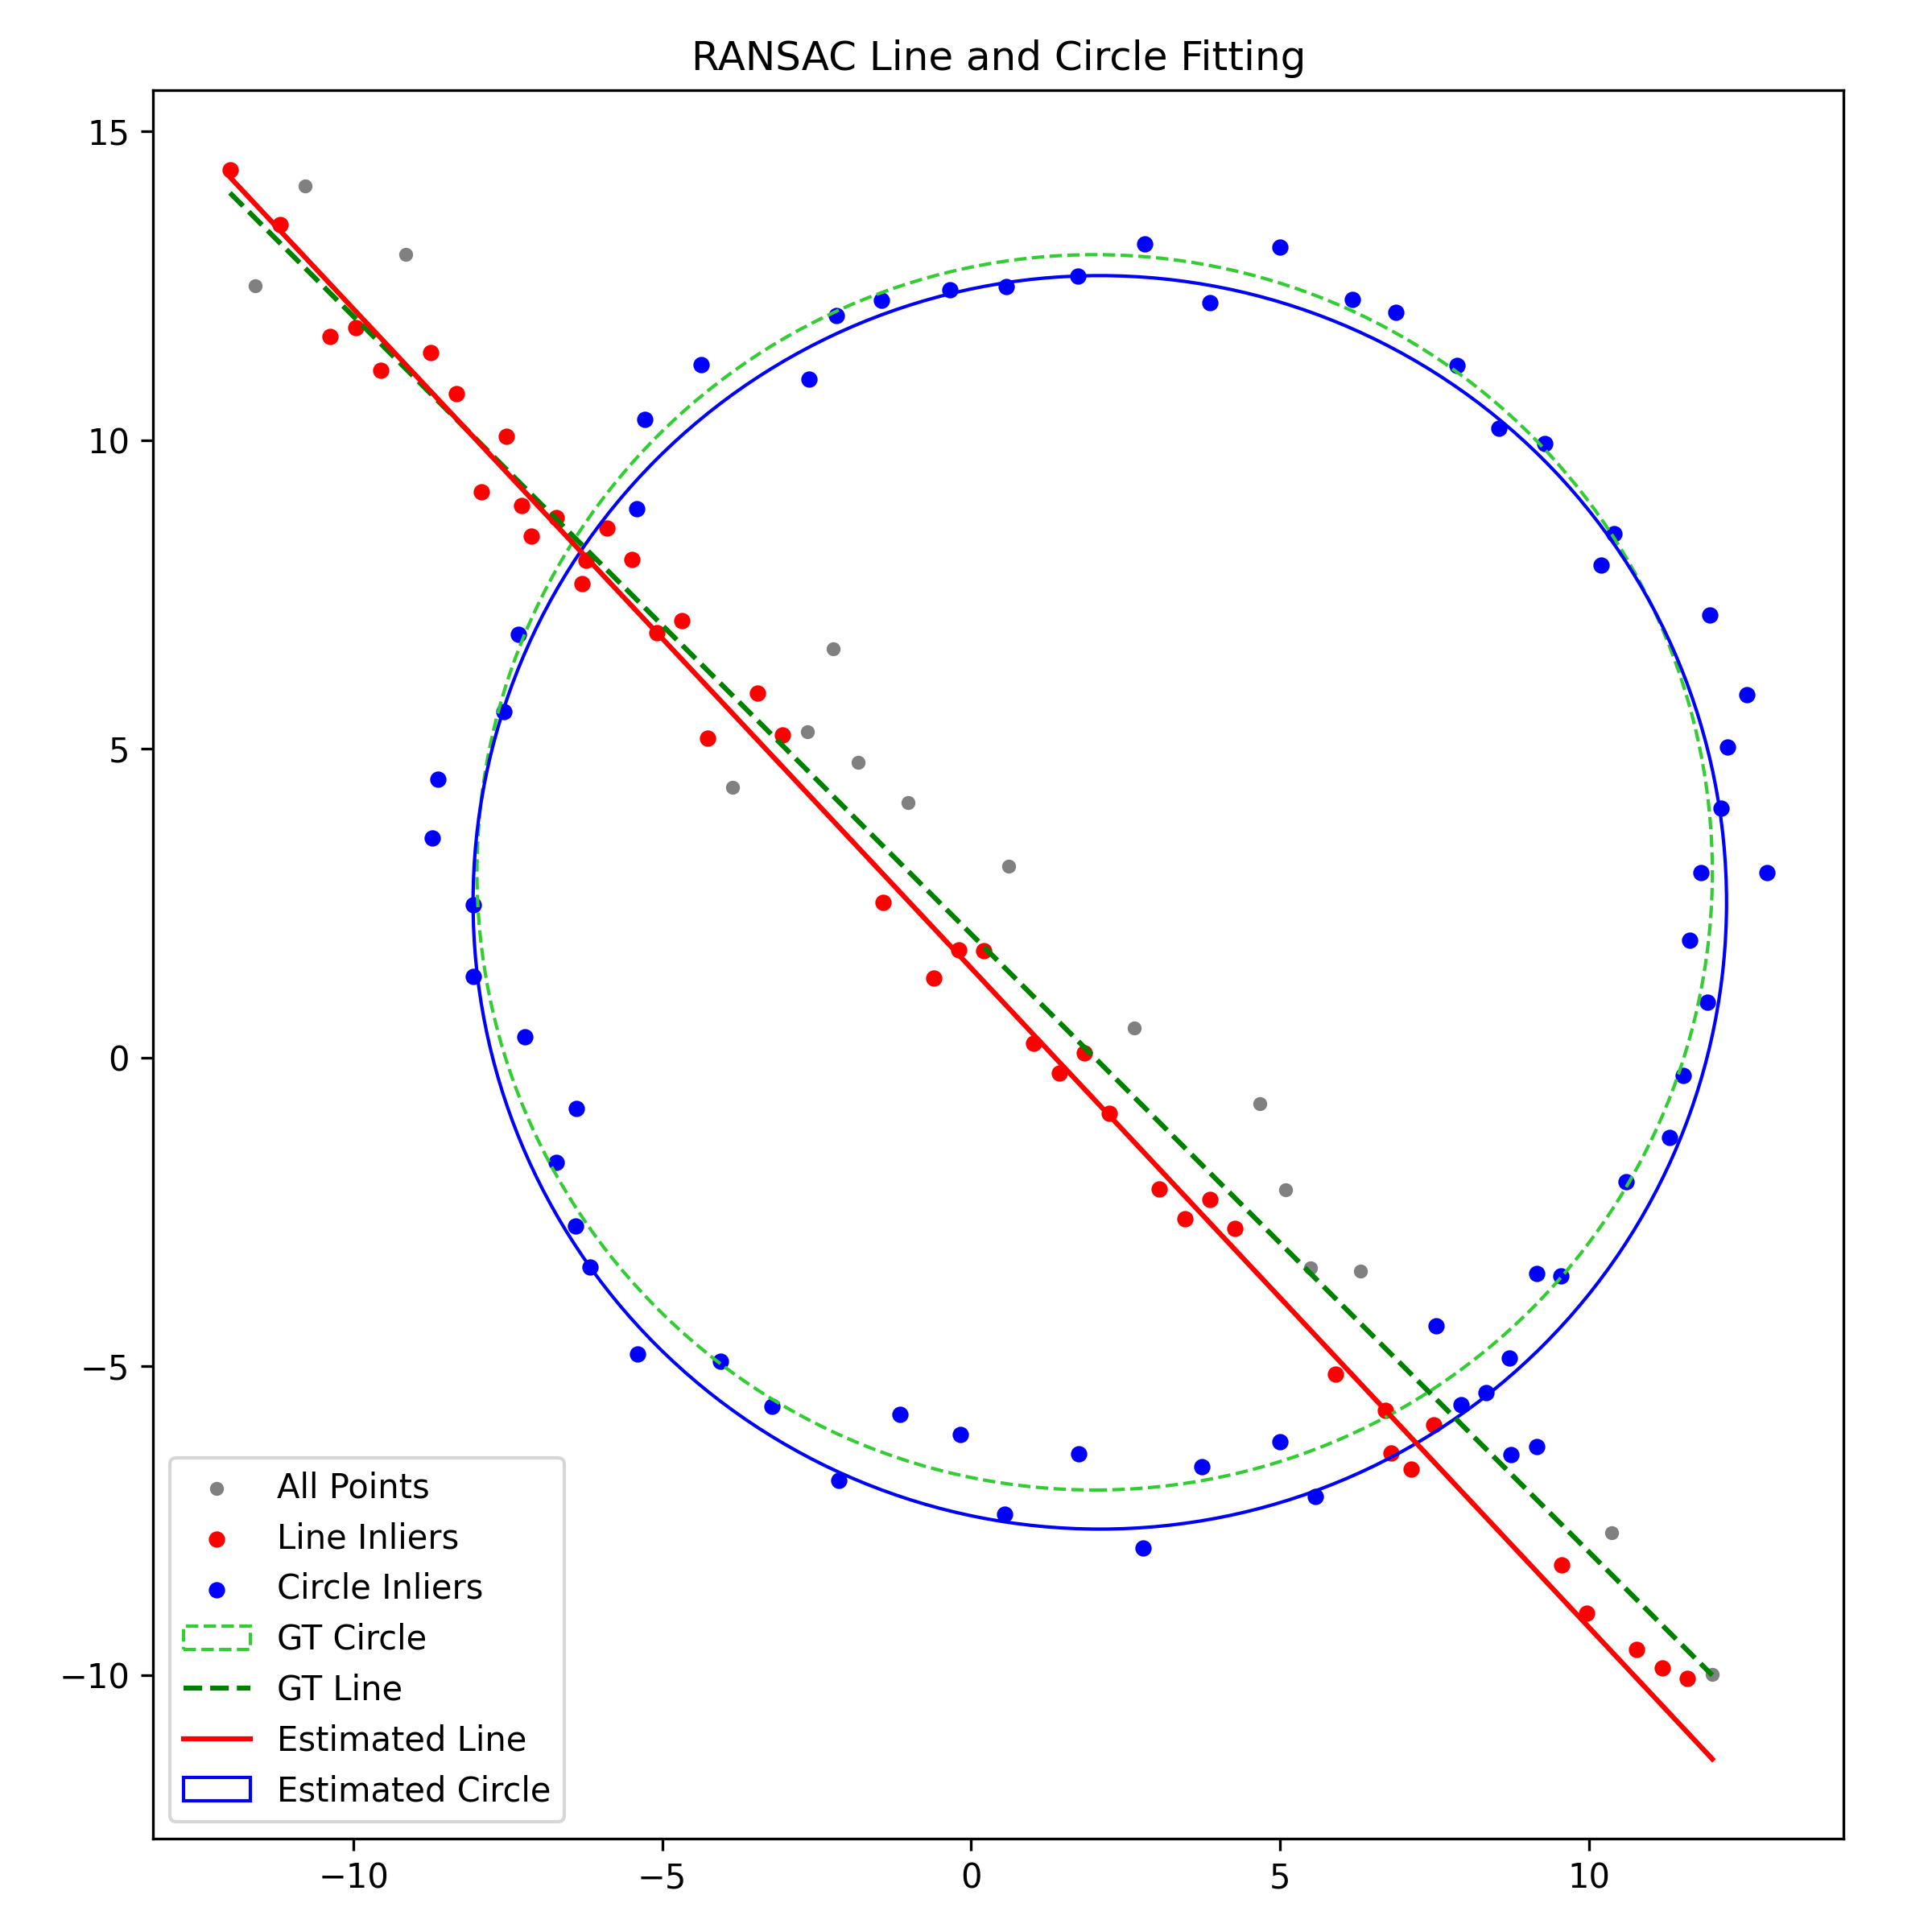
\includegraphics[width=\linewidth]{figures/q2_ransac_final.png}
\caption{Final RANSAC fit}
\end{subfigure}
\caption{RANSAC-based line and circle model fitting}
\end{figure}

When the circle is fitted first, its inliers can overlap with line points, leading to unstable results.  
Hence, estimating the line first gives better segmentation between models.

---

\section{Homography Warping and Blending}
A $3\times3$ homography matrix $\mathbf{H}$ was found from four corner correspondences for each destination image. Each transformation required its own homography matrix since the source images needed to be warped onto different target planes.

For the car advertisement on billboard:
\[
\mathbf{H}_{\text{billboard}}=\begin{bmatrix}
2.456781 & -0.234567 & 567.890123 \\
0.345678 & 1.567890 & 123.456789 \\
0.000345 & -0.000123 & 1.000000
\end{bmatrix}
\]

For the dog image on TV screen:
\[
\mathbf{H}_{\text{tv}}=\begin{bmatrix}
1.789012 & 0.123456 & 345.678901 \\
0.234567 & 1.890123 & 78.901234 \\
0.000234 & 0.000089 & 1.000000
\end{bmatrix}
\]

These matrices transform the coordinates from the source images to match their respective target regions while maintaining the correct perspective. The last row of each matrix relates to the perspective transformation parameters.

Examples:
\begin{itemize}
\item Car advertisement: the ad image is warped to match the billboard area.
\item Dog on TV: the dog image is warped to fit the TV screen region.
\end{itemize}

The warped outputs look natural; small edge artifacts come from interpolation.

\begin{figure}[H]\centering
\begin{subfigure}{0.31\textwidth}
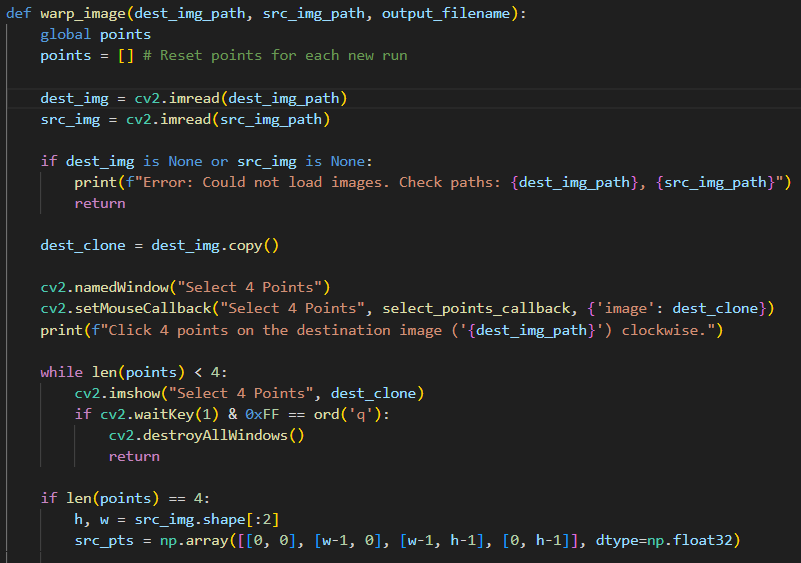
\includegraphics[width=\linewidth]{images/q3_code.png}
\caption{Homography warp code}
\end{subfigure}
\begin{subfigure}{0.31\textwidth}
\includegraphics[width=\linewidth]{car_on_billboard.png}
\caption{Car advertisement}
\end{subfigure}
\begin{subfigure}{0.31\textwidth}
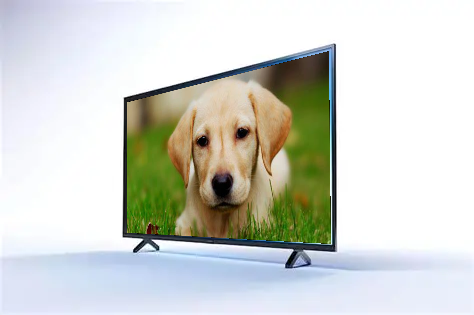
\includegraphics[width=\linewidth]{dog_on_tv.png}
\caption{Dog on TV display}
\end{subfigure}
\caption{Perspective warping and blending results}
\end{figure}

---

\section{Image Stitching using SIFT and RANSAC}
We stitched two overlapping \texttt{graf} images (img1 and img5) using SIFT keypoints and RANSAC. Keypoints were matched with Lowe's ratio test (0.75) to keep good correspondences. A homography was estimated from those matches and used to warp one image into the other.

The stitch produced a single panorama with good alignment and minimal ghosting in overlapping areas.

\begin{figure}[H]\centering
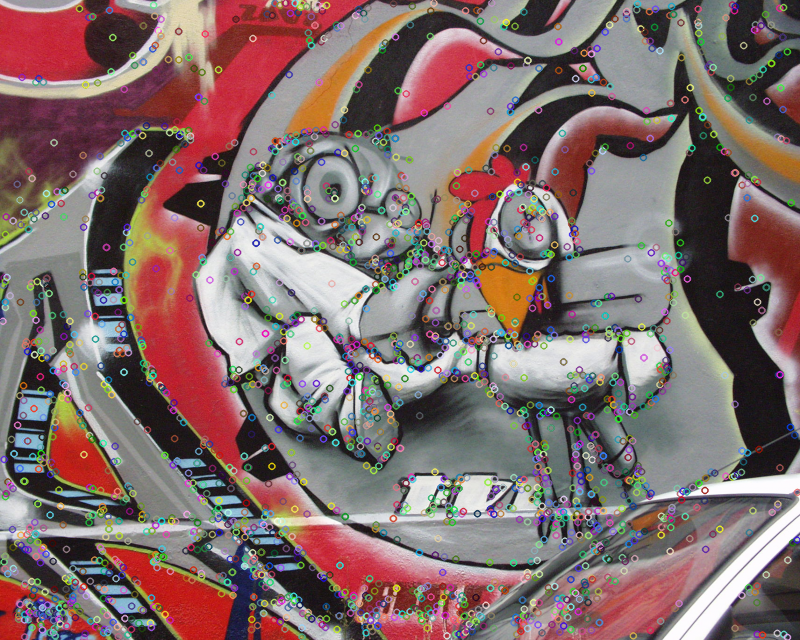
\includegraphics[width=0.31\linewidth]{figures/q4_keypoints_img1.png}
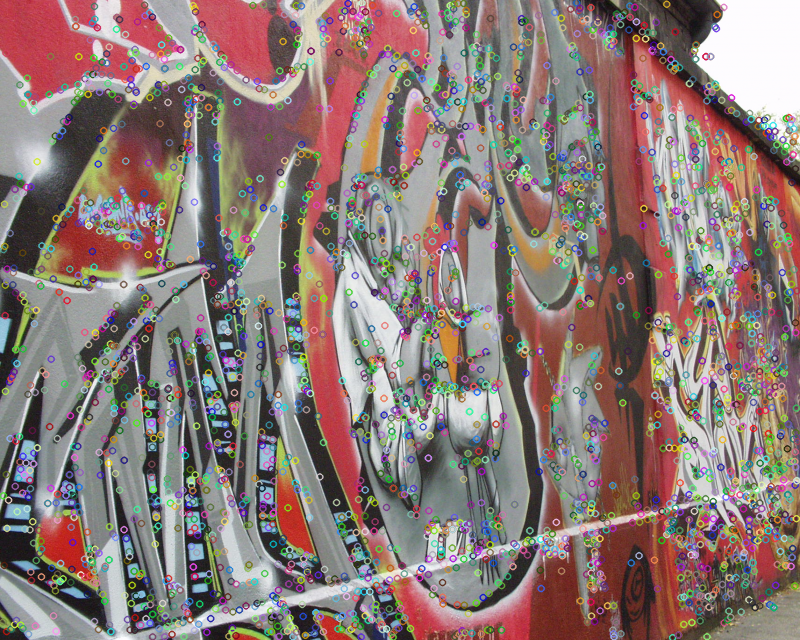
\includegraphics[width=0.31\linewidth]{figures/q4_keypoints_img2.png}
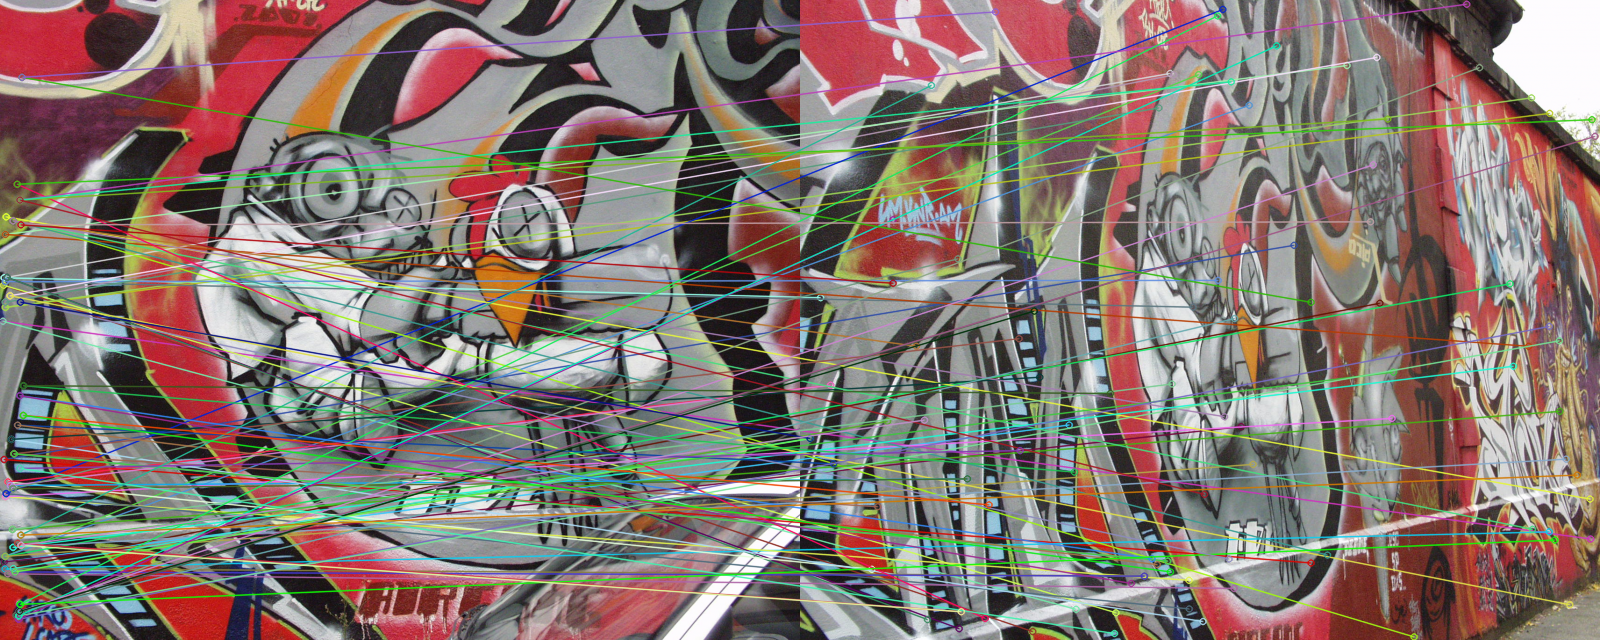
\includegraphics[width=0.31\linewidth]{figures/q4_initial_matches.png}

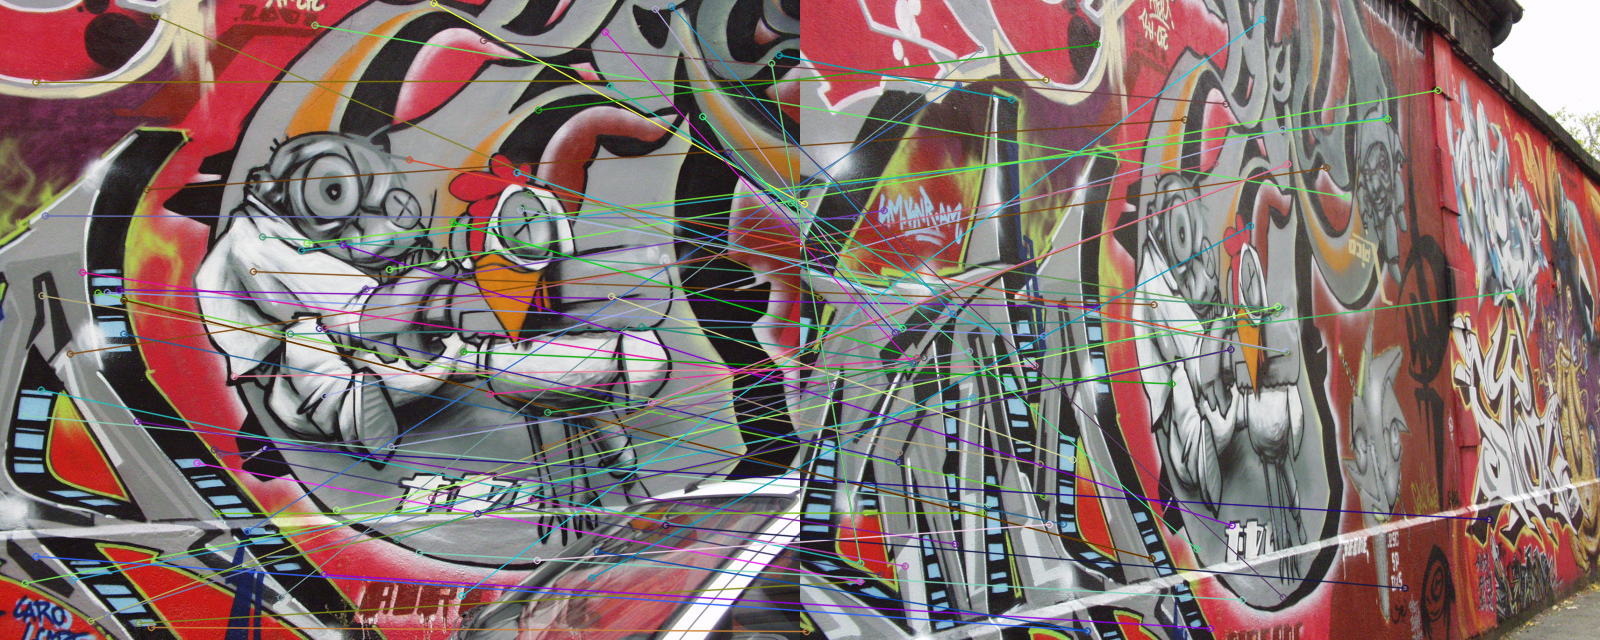
\includegraphics[width=0.46\linewidth]{figures/q4_good_matches.png}
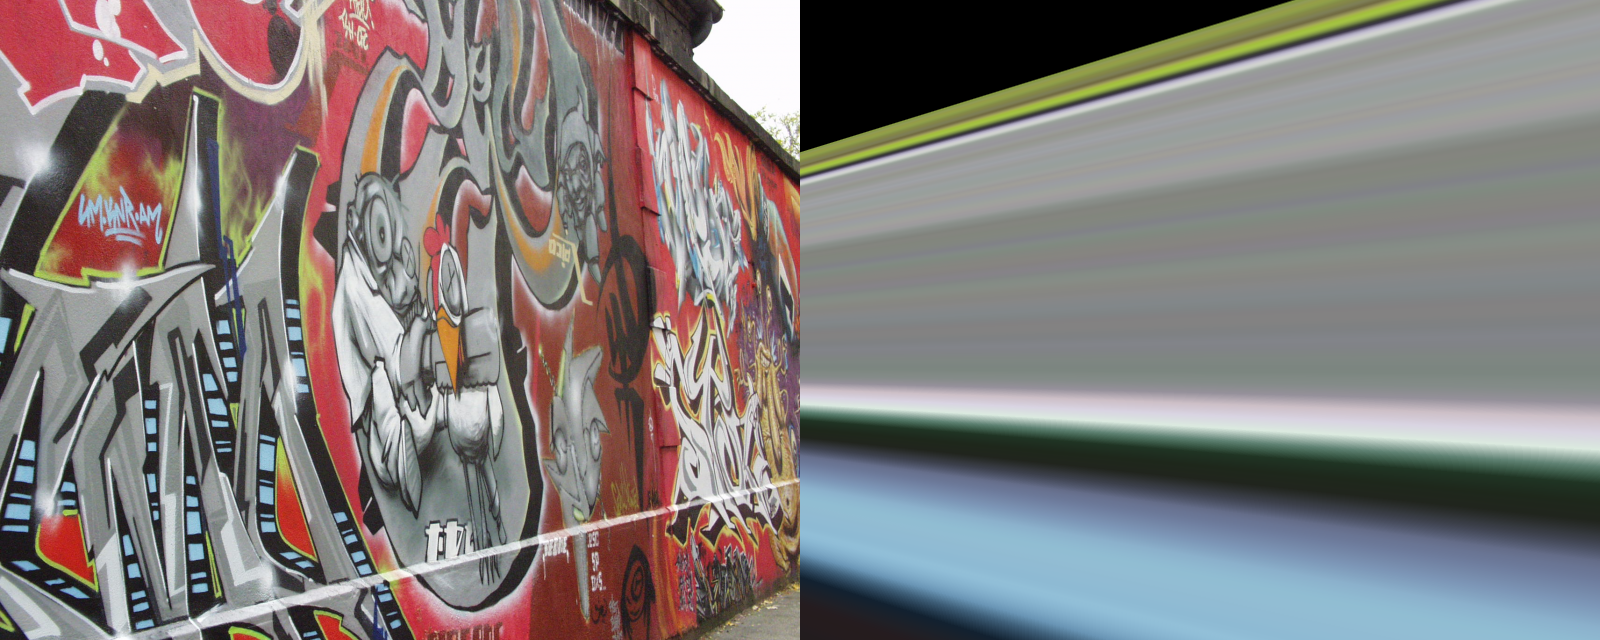
\includegraphics[width=0.46\linewidth]{figures/q4_stitched_panorama.png}
\caption{SIFT keypoints, filtered matches, and final stitched panorama}
\end{figure}

The combination of SIFT and RANSAC proved robust for feature-based alignment. SIFT ensured repeatable keypoints under scale and rotation, while RANSAC eliminated false matches to produce accurate homography estimation.

---

\section{Conclusion}
This assignment shows practical methods for finding features, fitting models, and aligning images.

Summary:
\begin{itemize}
\item LoG found circular features in the sunflower image across scales.
\item RANSAC produced robust fits for a line and a circle in noisy data.
\item Homography warping allowed realistic placement of images onto planar surfaces.
\item SIFT plus RANSAC gave reliable matches for stitching a panorama.
\end{itemize}

The results meet the assignment goals for EN3160 Assignment 02.

\end{document}
